%! Author = UserHome
%! Date = 02.12.2024

\chapter{Algoritmy založené na DFS}

Táto kapitola sa zaoberá algoritmami, ktoré využívajú prehľadávanie do hĺbky (DFS) na riešenie problémov. Tieto algoritmy postupne skúmajú všetky možné riešenia a využívajú techniky, ako je dopredná kontrola a backtracking, na optimalizáciu procesu hľadania riešení.

\section*{DFS}
File: solver/dfs.py

DFS je vyhľadávací algoritmus v strome alebo grafe, ktorý vždy vyberá najhlbší uzol (pomocou štruktúry Zasobník). Tento algoritmus má nízke pamäťové nároky, ale časová zložitosť je veľmi vysoká. Na riešenie problému n kráľovien musíme definovať naše uzly stromu (stavy), ktoré bude algoritmus prehľadávať. V našom prípade je stav definovaný ako ľubovoľné usporiadanie n kráľovien na šachovnici.

Od iných algoritmov sa líši tým, že  nerozlišuje a nijak nevyhodnocuje stavy šachovnice, pozná len počiatočný a cieľový stavy. V našom prípade algoritmus začína s prázdnou šachovnicou a hľadá stav (cieľový), v ktorom sú bezpečne umiestnené všetky dámy na šachovnici.
\begin{table}[h!]
    \centering
    \begin{tabular}{|l|c|c|c|c|}
        \hline
        \textbf{Problem Size} & \textbf{Time (Sec)} & \textbf{Nodes Expanded} & \textbf{Solved} \\
        \hline
        4 & 0.0007 & 154 & True \\
        8 & 4.4990 & 1,485,548 & True \\
        9 & 37.1991 & 14,226,687 & True \\
        \hline
    \end{tabular}
    \caption{Výsledky algoritmu DFS}
    \label{tab:dfs_results}
\end{table}
\section*{Spätné prehľadávanie}
File: solver/dfs\_backtracking.py

Algoritmus spätného prehľadávania je populárna metóda, ktorá používa rovnakú stratégiu prehľadávania stavov ako algoritmus DFS, ale vyradí tie stavy, ktoré nespĺňajú podmienku konzistencie pre konkrétny problém. Jeho kľúčovou vlastnosťou je postupné overovanie tejto podmienky. Napríklad v probléme s n dámami to znamená, že sa pred umiestnením dámy overí, či na vybranej pozícii nebude napadnutá.

\begin{table}[h!]
  \centering
  \begin{tabular}{|c|c|c|c|}
    \hline
    \textbf{Problem Size} & \textbf{Time (Sec)} & \textbf{Nodes Expanded} & \textbf{Solved} \\
    \hline
    4 & 0.0002 & 8 & True \\
    8 & 0.0046 & 113 & True \\
    9 & 0.0019 & 41 & True \\
    16 & 0.6483 & 10,052 & True \\
    20 & 17.6723 & 199,635 & True \\
    25 & 6.7871 & 48,683 & True \\
    \hline
  \end{tabular}
  \caption{Výsledky spätného prehľadávania}
  \label{tab:backtracking_basic_results}
\end{table}

Na ďalšiu optimalizáciu spätného prehľadávania, konkrétne na zníženie počtu krokov, môžeme zvážiť zmenu poradia výberu premenných a hodnôt ich domén.
Na použitie týchto metód je potrebné jasne sformulovať problém.

Formulácia problému:
\begin{itemize}
    \item \textbf{Premenne problému:} $n$ kráľovien, ktoré predstavujú riadok na šachovnici.
    \item \textbf{Doména hodnôt premenných:} $\{0, \dots, n - 1\}$, čo predstavuje stĺpec na šachovnici.
\end{itemize}

\section*{MRV pri spätnom prehľadávaní}
Algoritmus spätného prehľadávania zvyčajne vyberá premenné problému v náhodnom poradí (v našom prípade postupne, počnúc horným riadkom, prvou dámou). Tento prístup nie je vždy optimálny a na jeho zlepšenie možno použiť metódu minimálnych zostávajúcich hodnôt.
Logika tohto prístupu spočíva v tom, že sa najprv vyberú premenné, ktoré s najväčšou pravdepodobnosťou spôsobia problém v budúcnosti, čím sa implementuje stratégia fail-first. V praxi to znamená výber kráľovnej, ktorá má v doméne najmenší počet platných hodnôt (stĺpce, ktoré nie sú napadnuté).
\section*{LCV pri spätnom prehľadávaní}
Podobne ako pri výbere premennej, algoritmus spätného prehľadávania vyberá hodnoty domény postupne. Existuje však aj iný prístup, ktorý sa vola Najmenej obmedzujúca hodnota (LCV). V praxi to znamena, že hodnoty domén sa budu vyhodnocovať podľa počtu konfliktov, ktoré spôsobujú, a vyberie sa tá, ktorá spôsobuje ich najmenej. Logikou daného pristupu je zachovanie maximálnej flexibility pri výbere hodnôt domén ostatných premenných, čo vykazuje aj dobre výsledky.

\begin{table}[h!]
  \centering
  \begin{tabular}{|c|c|c|c|}
    \hline
    \textbf{Problem Size} & \textbf{Time (Sec)} & \textbf{Nodes Expanded} & \textbf{Solved} \\
    \hline
    8   & 0.0048 & 56    & TRUE \\
    9   & 0.0048 & 39    & TRUE \\
    16  & 0.1873 & 575   & TRUE \\
    30  & 0.4972 & 98    & TRUE \\
    50  & 20.6819 & 2554  & TRUE \\
    70  & 55.4207 & 2355  & TRUE \\
    80  & 55.5211 & 322   & TRUE \\
    90  & 2258.5207 & 57989 & TRUE \\
    100 & 162.6291 & 306   & TRUE \\
    \hline
  \end{tabular}
  \caption{Výsledky spätného prehľadávania pri použití MRV a LCV súčasne}
  \label{tab:backtracing_extended_results}
\end{table}

\section*{Dopredná kontrola}
File: solver/forward\_checking.py\par

Domény pre tento problém sú definované tak, že každá kráľovná je reprezentovaná ako premenná, ktorá sa nachádza v konkrétnom riadku šachovnice. Doména tejto premennej je množina možných pozícií, ktoré môže kráľovná zaujať v príslušnom riadku. V prípade 4x4 šachovnice má každá kráľovná na začiatku 4 možné hodnoty (stĺpce od 0 do 3) ako je znázornené na obrázku \ref{fig:forward-checking-zero-step}. Akonáhle sa však jedna z kráľovien umiestni na konkrétnu pozíciu, zvyšné hodnoty v doméne sú zredukované na základe konfliktov s ostatnými kráľovnami ako je znázornené na obrázku \ref{fig:forward-checking-first-step}.\par

Ak po umiestnení ďalšej dámy existuje aspoň jeden riadok, do ktorého nie je možné umiestniť dámu bez konfliktu ako je znázornené na obrázku~\ref{fig:forward-checking-empty-domain}, potom sa ďalšia dáma neumiestni a algoritmus vykoná krok späť .


\begin{figure}
    \centering
    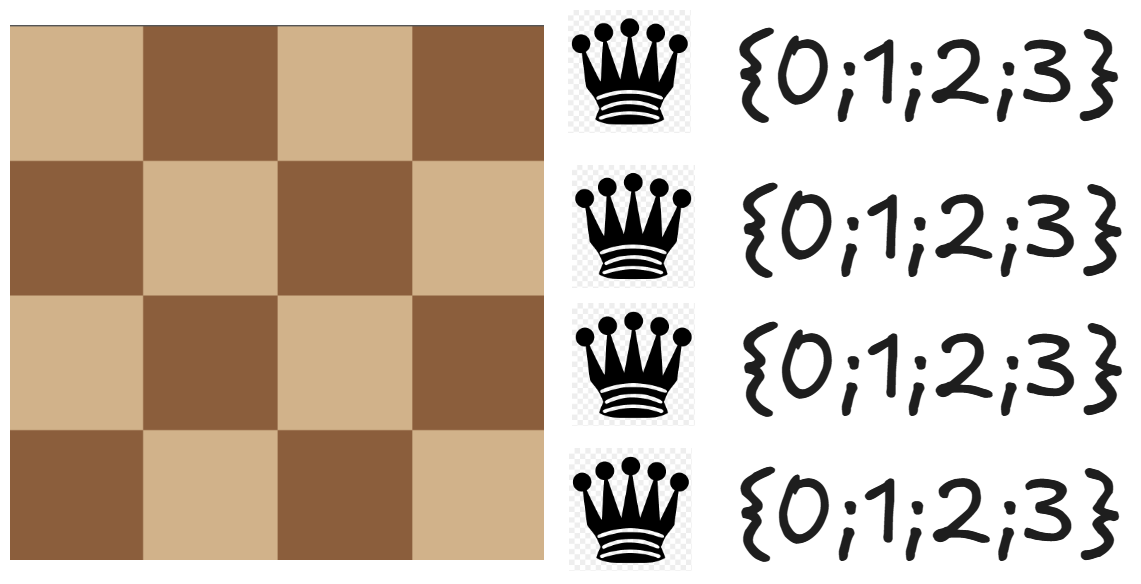
\includegraphics[width=0.7\textwidth]{figs/forward-checking/forward-checking-zero-step}
    \caption{Počiatočný stav doprednej kontroly}
    \label{fig:forward-checking-zero-step}
\end{figure}
\begin{figure}
    \centering
    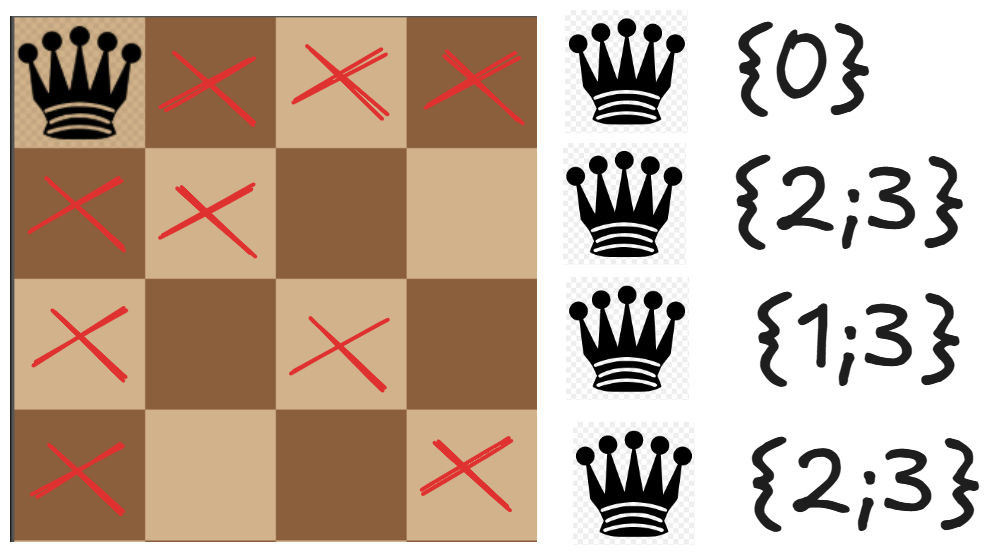
\includegraphics[width=0.6\textwidth]{figs/forward-checking/forward-checking-first-step}
    \caption{Prvý krok doprednej kontroly}
    \label{fig:forward-checking-first-step}
\end{figure}
\begin{figure}
    \centering
    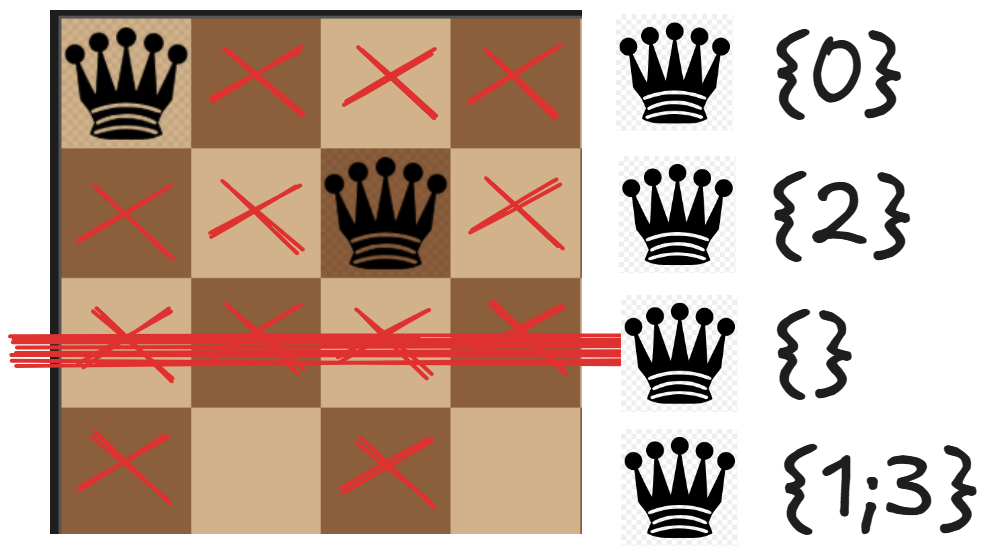
\includegraphics[width=0.6\textwidth]{figs/forward-checking/forward-checking-empty-domain}
    \caption{Prázdna doména v doprednej kontrole}
    \label{fig:forward-checking-empty-domain}
\end{figure}

\section{MRV v doprednej kontroe}
Riadok, v ktorom bude umiestnená ďalšia dáma, sa vyberie ako riadok, v ktorom má dáma najmenší počet možných pozícií. Ako je znázornené na obrázku \ref{fig:forward-checking-mrv} prvý riadok\footnote{Číslovanie začína od 0.} má najmenší počet možností umiestnenia kráľovnej, takže kráľovná bude umiestnená na ňom.
\begin{figure}
    \centering
    
\includegraphics[width=1\textwidth]{figs/forward-checking/forward-checking-mrv}
    \caption{Výber riadku pri doprednej kontrole pomocou MRV}
    \label{fig:forward-checking-mrv}
\end{figure}

\section{LCV v doprednej kontrole}
Po výbere riadku pomocou MRV sa vyberie stĺpec, v ktorom bude umiestnená kráľovná. Vyberie sa pozícia, na ktorej kráľovná vytvorí najmenší možný počet nových konfliktov. Na obrázku \ref{fig:forward-checking-lcv} prvá kráľovná vytvorí 2 nové konflikty a druhá vytvorí 3 konflikty.
\begin{figure}
    \centering
    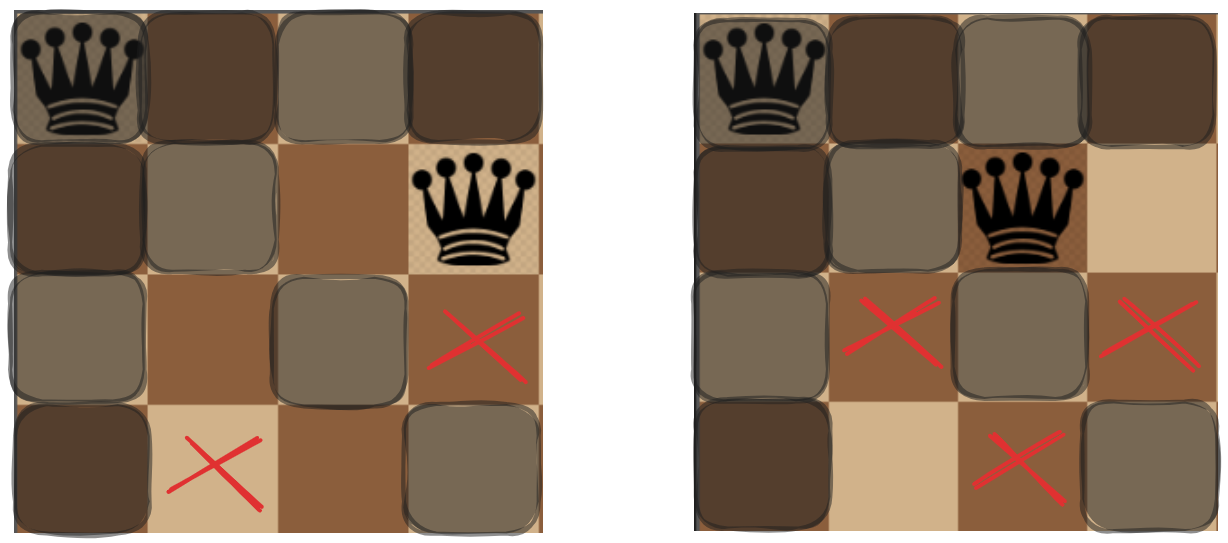
\includegraphics[width=0.8\textwidth]{figs/forward-checking/forward-checking-lcv}
    \caption{Výber stĺpca pri doprednej kontroly pomocou LCV}
    \label{fig:forward-checking-lcv}
\end{figure}

\begin{table}[h!]
  \centering
  \begin{tabular}{|c|c|c|c|}
    \hline
    \textbf{Problem Size} & \textbf{Time (Sec)} & \textbf{Nodes Expanded} & \textbf{Solved} \\
    \hline
    8   & 0.0145368576 & 39    & TRUE \\
    9   & 0.0107254982 & 21    & TRUE \\
    16  & 0.3472878933 & 332   & TRUE \\
    30  & 0.2026946545 & 68    & TRUE \\
    50  & 7.198326826  & 902   & TRUE \\
    70  & 13.18685579  & 1014  & TRUE \\
    80  & 3.904132605  & 207   & TRUE \\
    90  & 525.7122047  & 21536 & TRUE \\
    100 & 5.13761878   & 175   & TRUE \\
    \hline
  \end{tabular}
  \caption{Výsledky doprednej kontroly pri použití MRV a LCV súčasne}
  \label{tab:forward_checking_extended_results}
\end{table}

\section{Zhrnutie}

Grafy \ref{fig:size} a \ref{fig:time} zobrazujú výsledky z tabuliek uvedených pri každej metóde. Vyplýva z nich niekoľko zaujímavých záverov. Algoritmus DFS je výrazne horší z hľadiska spotrebovaného času aj počtu navštívených uzlov. Aj pri malých veľkostiach problémov je jasne viditeľná jeho nevýhoda.\par
\begin{figure}
    \centering
    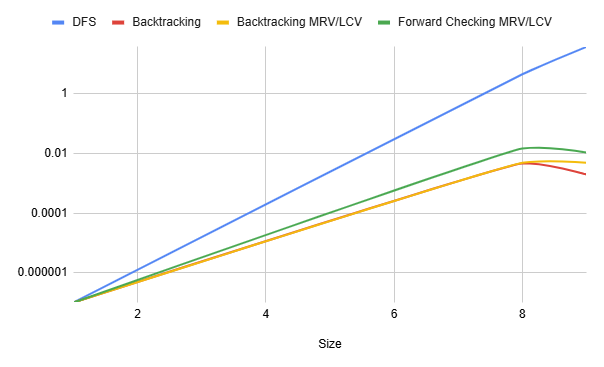
\includegraphics[width=1\textwidth]{figs/img_1}
    \caption{Porovnanie z pohľadu časovej náročnosti}
    \label{fig:time}
\end{figure}
\begin{figure}
    \centering
    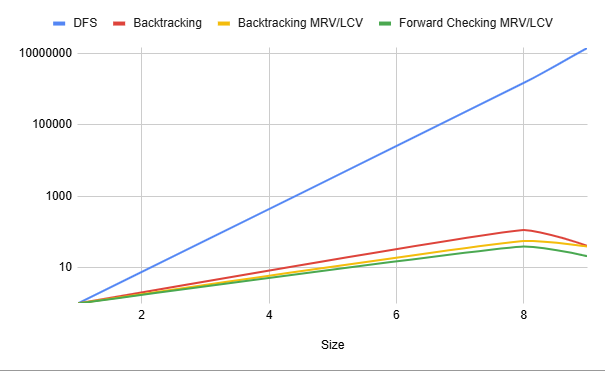
\includegraphics[width=1\textwidth]{figs/img}
    \caption{Porovnanie z pohľadu počtu navštívených stavov}
    \label{fig:size}
\end{figure}
Ďalej je vhodné porovnať doprednú kontrolu a spätne prehľadávanie (s MRV, LCV). Je zaujímavé, že kvôli svojej zložitosti algoritmus doprednej kontroly síce stráca na čase, ale rozširuje menej uzlov. Ak sa pozriete na väčší graf~\ref{fig:last}, dopredná kontrola (forward checking) je lepšia aj z hľadiska spotreby času.
\begin{figure}
    \centering
    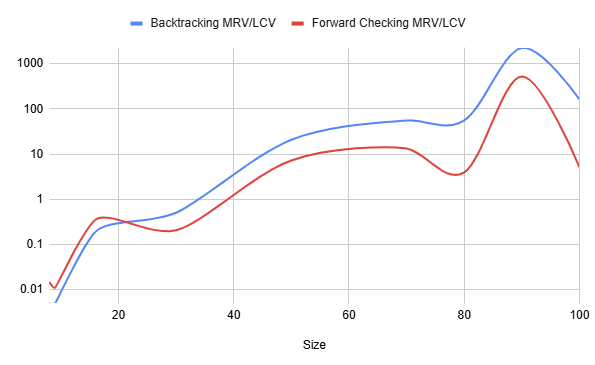
\includegraphics[width=1\textwidth]{figs/img_2}
    \caption{Porovnanie doprednej konroly a spetneho prehľadávania z pohľadu časovej náročnosti}
    \label{fig:last}
\end{figure}
